\documentclass[tikz,border=8pt]{standalone}
% Shared look for every TikZ diagram. Load with % Shared look for every TikZ diagram. Load with % Shared look for every TikZ diagram. Load with \input{../../tools/tikz-style.tex}
\usepackage[T1]{fontenc}
\usepackage{lmodern}
\renewcommand{\sfdefault}{lmr}  % diagrams use the same serif as the text
\usetikzlibrary{arrows.meta, positioning, shapes.geometric, calc, fit, backgrounds}
\definecolor{cblue}{HTML}{4C78A8}
\definecolor{corange}{HTML}{F58518}
\definecolor{cgreen}{HTML}{54A24B}
\definecolor{cred}{HTML}{E45756}
\definecolor{cpurple}{HTML}{B279A2}
\definecolor{cgrey}{HTML}{6B6B6B}
\tikzset{
  every picture/.style={font=\sffamily, line width=1.2pt},
  box/.style={draw=#1, fill=#1!12, rounded corners=4pt, align=center, inner sep=7pt, minimum height=1.1cm},
  box/.default=cgrey,
  arrow/.style={-{Stealth[length=3mm]}, draw=cgrey, line width=1.4pt},
  title/.style={font=\sffamily\bfseries\Large},
  note/.style={font=\sffamily\small, text=cgrey, align=center},
}
\AtBeginDocument{\hyphenpenalty=10000 \exhyphenpenalty=10000}

\usepackage[T1]{fontenc}
\usepackage{lmodern}
\renewcommand{\sfdefault}{lmr}  % diagrams use the same serif as the text
\usetikzlibrary{arrows.meta, positioning, shapes.geometric, calc, fit, backgrounds}
\definecolor{cblue}{HTML}{4C78A8}
\definecolor{corange}{HTML}{F58518}
\definecolor{cgreen}{HTML}{54A24B}
\definecolor{cred}{HTML}{E45756}
\definecolor{cpurple}{HTML}{B279A2}
\definecolor{cgrey}{HTML}{6B6B6B}
\tikzset{
  every picture/.style={font=\sffamily, line width=1.2pt},
  box/.style={draw=#1, fill=#1!12, rounded corners=4pt, align=center, inner sep=7pt, minimum height=1.1cm},
  box/.default=cgrey,
  arrow/.style={-{Stealth[length=3mm]}, draw=cgrey, line width=1.4pt},
  title/.style={font=\sffamily\bfseries\Large},
  note/.style={font=\sffamily\small, text=cgrey, align=center},
}
\AtBeginDocument{\hyphenpenalty=10000 \exhyphenpenalty=10000}

\usepackage[T1]{fontenc}
\usepackage{lmodern}
\renewcommand{\sfdefault}{lmr}  % diagrams use the same serif as the text
\usetikzlibrary{arrows.meta, positioning, shapes.geometric, calc, fit, backgrounds}
\definecolor{cblue}{HTML}{4C78A8}
\definecolor{corange}{HTML}{F58518}
\definecolor{cgreen}{HTML}{54A24B}
\definecolor{cred}{HTML}{E45756}
\definecolor{cpurple}{HTML}{B279A2}
\definecolor{cgrey}{HTML}{6B6B6B}
\tikzset{
  every picture/.style={font=\sffamily, line width=1.2pt},
  box/.style={draw=#1, fill=#1!12, rounded corners=4pt, align=center, inner sep=7pt, minimum height=1.1cm},
  box/.default=cgrey,
  arrow/.style={-{Stealth[length=3mm]}, draw=cgrey, line width=1.4pt},
  title/.style={font=\sffamily\bfseries\Large},
  note/.style={font=\sffamily\small, text=cgrey, align=center},
}
\AtBeginDocument{\hyphenpenalty=10000 \exhyphenpenalty=10000}

\begin{document}
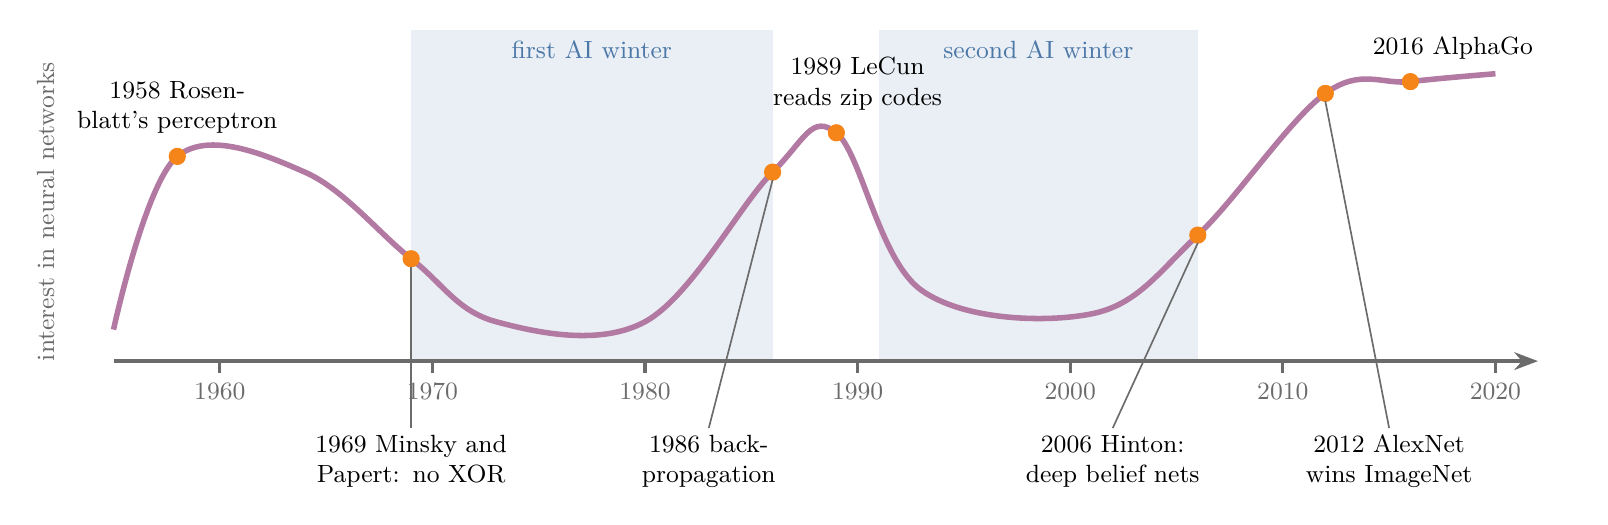
\begin{tikzpicture}[x=0.27cm, y=1cm, ev/.style={note, text=black, text width=3.0cm, font=\sffamily\small}]
  % year axis 1955..2020 -> x = year-1955
  \fill[cblue!12] (14,0) rectangle (31,4.2); \node[note, text=cblue] at (22.5,3.95) {first AI winter};
  \fill[cblue!12] (36,0) rectangle (51,4.2); \node[note, text=cblue] at (43.5,3.95) {second AI winter};
  \draw[arrow] (0,0) -- (67,0);
  \foreach \yr in {1960,1970,1980,1990,2000,2010,2020} {\draw[cgrey] (\yr-1955,0) -- ++(0,-0.15); \node[note, below] at (\yr-1955,-0.15) {\yr};}
  \node[note, rotate=90] at (-3.2,1.9) {interest in neural networks};
  \draw[cpurple, line width=2pt] plot[smooth, tension=0.6] coordinates {(0,0.4) (3,2.6) (9,2.4) (14,1.3) (18,0.5) (25,0.5) (31,2.4) (34,2.9) (38,0.9) (46,0.6) (51,1.6) (57,3.4) (61,3.55) (65,3.65)};
  \foreach \x/\y in {3/2.6, 14/1.3, 31/2.4, 34/2.9, 51/1.6, 57/3.4, 61/3.55} \node[circle, fill=corange, inner sep=2.2pt] at (\x,\y) {};
  \node[ev, anchor=south] at (3,2.75) {1958 Rosenblatt's perceptron};
  \node[ev, anchor=north] at (14,-0.8) {1969 Minsky and Papert: no XOR};
  \draw[cgrey, line width=0.6pt] (14,-0.85) -- (14,1.2);
  \node[ev, anchor=north] at (28,-0.8) {1986 backpropagation};
  \draw[cgrey, line width=0.6pt] (28,-0.85) -- (31,2.3);
  \node[ev, anchor=south] at (35,3.05) {1989 LeCun reads zip codes};
  \node[ev, anchor=north] at (47,-0.8) {2006 Hinton: deep belief nets};
  \draw[cgrey, line width=0.6pt] (47,-0.85) -- (51,1.5);
  \node[ev, anchor=north] at (60,-0.8) {2012 AlexNet wins ImageNet};
  \draw[cgrey, line width=0.6pt] (60,-0.85) -- (57,3.3);
  \node[ev, anchor=south] at (63,3.7) {2016 AlphaGo};
\end{tikzpicture}
\end{document}
